% Options for packages loaded elsewhere
\PassOptionsToPackage{unicode}{hyperref}
\PassOptionsToPackage{hyphens}{url}
%
\documentclass[
]{book}
\usepackage{amsmath,amssymb}
\usepackage{lmodern}
\usepackage{iftex}
\ifPDFTeX
  \usepackage[T1]{fontenc}
  \usepackage[utf8]{inputenc}
  \usepackage{textcomp} % provide euro and other symbols
\else % if luatex or xetex
  \usepackage{unicode-math}
  \defaultfontfeatures{Scale=MatchLowercase}
  \defaultfontfeatures[\rmfamily]{Ligatures=TeX,Scale=1}
\fi
% Use upquote if available, for straight quotes in verbatim environments
\IfFileExists{upquote.sty}{\usepackage{upquote}}{}
\IfFileExists{microtype.sty}{% use microtype if available
  \usepackage[]{microtype}
  \UseMicrotypeSet[protrusion]{basicmath} % disable protrusion for tt fonts
}{}
\makeatletter
\@ifundefined{KOMAClassName}{% if non-KOMA class
  \IfFileExists{parskip.sty}{%
    \usepackage{parskip}
  }{% else
    \setlength{\parindent}{0pt}
    \setlength{\parskip}{6pt plus 2pt minus 1pt}}
}{% if KOMA class
  \KOMAoptions{parskip=half}}
\makeatother
\usepackage{xcolor}
\IfFileExists{xurl.sty}{\usepackage{xurl}}{} % add URL line breaks if available
\IfFileExists{bookmark.sty}{\usepackage{bookmark}}{\usepackage{hyperref}}
\hypersetup{
  pdftitle={Reproducible Reporting},
  pdfauthor={Robert C. Cline, Sr., M.A., CPL},
  hidelinks,
  pdfcreator={LaTeX via pandoc}}
\urlstyle{same} % disable monospaced font for URLs
\usepackage{color}
\usepackage{fancyvrb}
\newcommand{\VerbBar}{|}
\newcommand{\VERB}{\Verb[commandchars=\\\{\}]}
\DefineVerbatimEnvironment{Highlighting}{Verbatim}{commandchars=\\\{\}}
% Add ',fontsize=\small' for more characters per line
\usepackage{framed}
\definecolor{shadecolor}{RGB}{248,248,248}
\newenvironment{Shaded}{\begin{snugshade}}{\end{snugshade}}
\newcommand{\AlertTok}[1]{\textcolor[rgb]{0.94,0.16,0.16}{#1}}
\newcommand{\AnnotationTok}[1]{\textcolor[rgb]{0.56,0.35,0.01}{\textbf{\textit{#1}}}}
\newcommand{\AttributeTok}[1]{\textcolor[rgb]{0.77,0.63,0.00}{#1}}
\newcommand{\BaseNTok}[1]{\textcolor[rgb]{0.00,0.00,0.81}{#1}}
\newcommand{\BuiltInTok}[1]{#1}
\newcommand{\CharTok}[1]{\textcolor[rgb]{0.31,0.60,0.02}{#1}}
\newcommand{\CommentTok}[1]{\textcolor[rgb]{0.56,0.35,0.01}{\textit{#1}}}
\newcommand{\CommentVarTok}[1]{\textcolor[rgb]{0.56,0.35,0.01}{\textbf{\textit{#1}}}}
\newcommand{\ConstantTok}[1]{\textcolor[rgb]{0.00,0.00,0.00}{#1}}
\newcommand{\ControlFlowTok}[1]{\textcolor[rgb]{0.13,0.29,0.53}{\textbf{#1}}}
\newcommand{\DataTypeTok}[1]{\textcolor[rgb]{0.13,0.29,0.53}{#1}}
\newcommand{\DecValTok}[1]{\textcolor[rgb]{0.00,0.00,0.81}{#1}}
\newcommand{\DocumentationTok}[1]{\textcolor[rgb]{0.56,0.35,0.01}{\textbf{\textit{#1}}}}
\newcommand{\ErrorTok}[1]{\textcolor[rgb]{0.64,0.00,0.00}{\textbf{#1}}}
\newcommand{\ExtensionTok}[1]{#1}
\newcommand{\FloatTok}[1]{\textcolor[rgb]{0.00,0.00,0.81}{#1}}
\newcommand{\FunctionTok}[1]{\textcolor[rgb]{0.00,0.00,0.00}{#1}}
\newcommand{\ImportTok}[1]{#1}
\newcommand{\InformationTok}[1]{\textcolor[rgb]{0.56,0.35,0.01}{\textbf{\textit{#1}}}}
\newcommand{\KeywordTok}[1]{\textcolor[rgb]{0.13,0.29,0.53}{\textbf{#1}}}
\newcommand{\NormalTok}[1]{#1}
\newcommand{\OperatorTok}[1]{\textcolor[rgb]{0.81,0.36,0.00}{\textbf{#1}}}
\newcommand{\OtherTok}[1]{\textcolor[rgb]{0.56,0.35,0.01}{#1}}
\newcommand{\PreprocessorTok}[1]{\textcolor[rgb]{0.56,0.35,0.01}{\textit{#1}}}
\newcommand{\RegionMarkerTok}[1]{#1}
\newcommand{\SpecialCharTok}[1]{\textcolor[rgb]{0.00,0.00,0.00}{#1}}
\newcommand{\SpecialStringTok}[1]{\textcolor[rgb]{0.31,0.60,0.02}{#1}}
\newcommand{\StringTok}[1]{\textcolor[rgb]{0.31,0.60,0.02}{#1}}
\newcommand{\VariableTok}[1]{\textcolor[rgb]{0.00,0.00,0.00}{#1}}
\newcommand{\VerbatimStringTok}[1]{\textcolor[rgb]{0.31,0.60,0.02}{#1}}
\newcommand{\WarningTok}[1]{\textcolor[rgb]{0.56,0.35,0.01}{\textbf{\textit{#1}}}}
\usepackage{longtable,booktabs,array}
\usepackage{calc} % for calculating minipage widths
% Correct order of tables after \paragraph or \subparagraph
\usepackage{etoolbox}
\makeatletter
\patchcmd\longtable{\par}{\if@noskipsec\mbox{}\fi\par}{}{}
\makeatother
% Allow footnotes in longtable head/foot
\IfFileExists{footnotehyper.sty}{\usepackage{footnotehyper}}{\usepackage{footnote}}
\makesavenoteenv{longtable}
\usepackage{graphicx}
\makeatletter
\def\maxwidth{\ifdim\Gin@nat@width>\linewidth\linewidth\else\Gin@nat@width\fi}
\def\maxheight{\ifdim\Gin@nat@height>\textheight\textheight\else\Gin@nat@height\fi}
\makeatother
% Scale images if necessary, so that they will not overflow the page
% margins by default, and it is still possible to overwrite the defaults
% using explicit options in \includegraphics[width, height, ...]{}
\setkeys{Gin}{width=\maxwidth,height=\maxheight,keepaspectratio}
% Set default figure placement to htbp
\makeatletter
\def\fps@figure{htbp}
\makeatother
\setlength{\emergencystretch}{3em} % prevent overfull lines
\providecommand{\tightlist}{%
  \setlength{\itemsep}{0pt}\setlength{\parskip}{0pt}}
\setcounter{secnumdepth}{5}
\usepackage{booktabs}
\ifLuaTeX
  \usepackage{selnolig}  % disable illegal ligatures
\fi
\usepackage[]{natbib}
\bibliographystyle{apalike}

\title{Reproducible Reporting}
\author{Robert C. Cline, Sr., M.A., CPL}
\date{2022-06-12}

\usepackage{amsthm}
\newtheorem{theorem}{Theorem}[chapter]
\newtheorem{lemma}{Lemma}[chapter]
\newtheorem{corollary}{Corollary}[chapter]
\newtheorem{proposition}{Proposition}[chapter]
\newtheorem{conjecture}{Conjecture}[chapter]
\theoremstyle{definition}
\newtheorem{definition}{Definition}[chapter]
\theoremstyle{definition}
\newtheorem{example}{Example}[chapter]
\theoremstyle{definition}
\newtheorem{exercise}{Exercise}[chapter]
\theoremstyle{definition}
\newtheorem{hypothesis}{Hypothesis}[chapter]
\theoremstyle{remark}
\newtheorem*{remark}{Remark}
\newtheorem*{solution}{Solution}
\begin{document}
\maketitle

{
\setcounter{tocdepth}{1}
\tableofcontents
}
\hypertarget{introduction}{%
\chapter{Introduction}\label{introduction}}

The scientific community has invested heavily in what is known as reproducible research to make their work reproducible for themselves and for other scientists wishing to replicate their studies to verify findings or explore the subject further. Reproducible research documents the research, making it both reproducible and verifiable. The technology available to create reproducible research is not limited to the scientific communty. Any individual or organization can utitlize this technology to make one's own reporting reproducible. The advantages of reproducible reporing are many, including organizing resources, and is used to automate the presentation of data analysis as data is compiled into a report for publication or review. Reproduciblity turns the process into an iterative process, so as the data changes, the reports themselves simply update automatically. Stated another way, much of our reporting and document preparation stays the same while only the data source changes. An example would be the preparation of oil and gas leases. Instead of a lease and offer letter being prepared for each Lessor, all packages can be prepared at once from one data source. The names, tracts, net minerals and bonus payments change for each lessor and for each project, only the data input changes. The process of producing the lease package is one print operation. Only the data changes. Very little time is used in preparing the lease package documents. This is where reproducible reporting has a great advantage over traditional reporting methods both in savings of time and money. The time savings is huge.

\hypertarget{usage}{%
\section{Usage}\label{usage}}

While replication is a fundamental tenet of science, it is grossley under utilized in business; especially the title business. The process of reporting in the title industry is expensive and time consuming. The process of interpreting title ownership requires ``hands-on'' review of title documentation and a knowledg of land law and contract law. However, the process of reporting the analysis can be shortened by utilizng the methodology of reproducible research. Reproducible reporting is a way of utilizing current technolgy to both create iterative types of reports and as a way to organize the title ownership data into easily managed data which can be maintained in a centralized database and updated as necessary.

\hypertarget{about-the-author}{%
\section{About the Author}\label{about-the-author}}

I, Robert C. Cline, Sr., hold a Masters Degree in Clinical Psychology from University of Houston-Clear Lake and I am an AAPL Certified Petroleum Landman. My family operated a sovereign title plant in Wharton Texas which was established by my granfather in 1890. I started working in that plant at age 11, a barefooted boy copying documents in the court house, developing and printing the images for the abstractor to compile into Abstracts and Title Certificates. I worked in that plant throughout my highschool years. After college, I attended a two year program at the University of Texas San Antonio Title School, earning a certificate in the title insurance industry. I was a licensed closing officer in the title plant and was a certified Title Examiner for several title insurance underwriters including Chicago Title Insurance Agency and Minisota Title Insurance Company, a title insurance underwriter, a position that, by industry standards, required a law degree and five years of practice of land title law. I was a member of the Texas Land Title Association and was a Title Plant Examiner for that organizatio, examining the records of title plants for adequacy and accuracy of title plants which had applied for membership in the association.

In 1976, I joined the brokerage firm of I. Jon Brook, Jr.~as a petroleum landman. In 1980, went to work for Clayton Williams, Jr.~in the Austin Chalk as a landman. Robert has had many clients over the years working as an Independent landman, managing title research for clients, managing due dilegence projects, leasing projects and seismic projects. Robert earned the master's degree while working full time in the oil and gas industry as a field landman. In 2010 to 2014, I managed the field operations for Fairways Exploration \& Production, LLC acquiring 10,000 leases covering 400,000 acres. At that same time, I manged a 100 square mile seismic acquisition project for that same company.

Today, I am still employed as a landman. During the downturn in the industry in 2014 to 2020, I used the time to study advanced statistics, learning methods to create reproducible research. I write R code, a statistical programming language and some python. I am proficient in Excel VBA, Power Query, Power Pivot and I create MS Access applications utilizing knowledge of VBA. I use GIS in both R programming language and with QGIS, both of which are open source applications.

\hypertarget{preview-book}{%
\section{Preview book}\label{preview-book}}

This proposal is written in the format of a book with the Bookdown package and is made available online in the form of an HTML document, PDF format, and as eBook publication. I intend to maintain a live preview which will update as I edit and change the document on an as-needed basis.

\begin{Shaded}
\begin{Highlighting}[]
\NormalTok{bookdown}\SpecialCharTok{::}\FunctionTok{serve\_book}\NormalTok{()}
\end{Highlighting}
\end{Shaded}

\begin{Shaded}
\begin{Highlighting}[]
\FunctionTok{citation}\NormalTok{(}\StringTok{"plotrix"}\NormalTok{)}
\end{Highlighting}
\end{Shaded}

\hypertarget{implications-for-reproducible-reporting}{%
\chapter{Implications for Reproducible Reporting}\label{implications-for-reproducible-reporting}}

In the world of scientific research, the purpose of data analysis is to make the data analysis as open and transparent as possible to be able to exactly reproduce any ofthe results that were produced by it \citep{andrewsChapterReproducibleData}.

The data analyis pipeline is analygous to analyzing land title ownership. Title analyis begins with acquiring title information from public records, documenting the title chain, reading the title chain and interpreting the chain of ownership and reducing the ownership into numerical quantities. Mineral titles often have many owners with multiple classes of ownership, from royalty interests, production interests, mineral interests, term interests, life estate and remainder interests, severed or interests in both surface and minerals. These interests are commonly referred to the ``bundle of sticks,'' meaning there are many classes of ownerships in the mineral and surface estates. A title report analyses these interests in the form of fractional ownership. Periods of ownership is important as well. In Nebraska, for example, an owner who has not documented a claim or had a transfer of interest in his severed mineral estate, is subject to claims of abandonment of the mineral interest by the surface owner. The individual owners interest must be compiled into an ownership report together with the contact information for each owner. Claims, such as Lis Pendens, delinquent taxes, pending County and District Court suits must be documented when reporting the status of the title for each owner.

\hypertarget{the-hypothetical-title-report}{%
\section{The Hypothetical Title Report}\label{the-hypothetical-title-report}}

Ownership reports are commonly lengthy and contain a lot of data depending on the complexity of the title. Areas where there is mineral production, the title can expected to be more complex and more time consuming to complete.

Creating title reports, like scientific research, is a multistep process. The Gantt chart below outlines a hypothetical number of days that it could take for each step in the process of compiling ownerhship reports.

\includegraphics{01-intro_files/figure-latex/nice-fig-1.pdf}

The Gantt chart lists six steps for the preparation of an ownership report and preparation of lease packages. I have had some mineral titles that had as few as one owner and as many as 350 owners. One never knows what title issues or how complex a title can be until one actually examines the title. The number of days chosen in the example below is simply a hypothetical case for illustration.\\
What can remain constanct is, the first four steps are relative in to steps 5 and six. That is, the number of days it takes to build the runsheet, analyize the title, calculate the owners' interests, is relative to the number of days it takes to build the report and prepare lease packages.

If for example one needs 15 days to get through calculating the owners' interests, one will need nearly that many days to build the report and prepare the lease packages. This is where reproducible reporting becomes an advantage.\\
Using the techniques of reproducible reporting, the time required for building the reports and preparing the lease packages is reduced from days to usually \emph{seconds}.

This advantage is multiple many fold if changes to the report must be made. Instead of re-writing a report, a simple change in the data for the report is made and the report is re-run in seconds.

\hypertarget{additional-benefits}{%
\subsection{Additional benefits}\label{additional-benefits}}

Mark Andrews \citep{andrewsChapterReproducibleData} emphasizes that reproducible data analysis is often motivated as a means of doing more high quality and robust data analyis as a way of quality control essential to measure, identify errors, increase regour and verify results and conclusions. Mark Andrews offers as an example, a \$9bn loss of investment bank JPMorgan in 2012 \citep{ExcelMostDangerous2021}. Keeping data in Excel also has created vulnerabilities. In 2020, the Public Health England lost Covid data as a result of using Excel to collect data. One expert commented ``even a high-school computing student would know that better alternatives {[}to Excel{]} exist. \ldots{} you wouldn't use XLS, nobody would do that'' \citep{ExcelWhyUsing2020}.

\hypertarget{summary-of-savings-with-reproducible-reporting}{%
\subsection{Summary of Savings with Reproducible Reporting}\label{summary-of-savings-with-reproducible-reporting}}

Each title examination is different from any other, no two titles are the same. No title examiner ever knows what awaits. Predicting the length of time to complete the title examination and compile the reporting is not feasible. But, as a rule of thumb the process of reporting is relative to the complexity of title. The more complex the title, the longer the process of preparing reports and lease packages. With reproducible reporting, the time process is reduced from the time it takes to examine the title to almost zero. Thus, by employing reproducible reporting, the savings in terms of time spent, is rougly one-half. Reproducible reporting saves about 50\% of the time it normally takes to produce the same result.

\hypertarget{laying-the-groundwork-for-project-management}{%
\subsection{Laying the groundwork for project management}\label{laying-the-groundwork-for-project-management}}

Creating the infrastructure for reproducible reporting requires an understanding of the software package R and parameterized reporting. The title persons do not need to process the output. With training, they can of course. But people preparing the title reports will typically do so using templates prepared in CSV format. CSV files, or if prefered XLSX files can be batched processed to create the output into MS Word, PDF or HTML files.

\hypertarget{cross}{%
\chapter{Cross-references}\label{cross}}

Cross-references make it easier for your readers to find and link to elements in your book.

\hypertarget{chapters-and-sub-chapters}{%
\section{Chapters and sub-chapters}\label{chapters-and-sub-chapters}}

There are two steps to cross-reference any heading:

\begin{enumerate}
\def\labelenumi{\arabic{enumi}.}
\tightlist
\item
  Label the heading: \texttt{\#\ Hello\ world\ \{\#nice-label\}}.

  \begin{itemize}
  \tightlist
  \item
    Leave the label off if you like the automated heading generated based on your heading title: for example, \texttt{\#\ Hello\ world} = \texttt{\#\ Hello\ world\ \{\#hello-world\}}.
  \item
    To label an un-numbered heading, use: \texttt{\#\ Hello\ world\ \{-\#nice-label\}} or \texttt{\{\#\ Hello\ world\ .unnumbered\}}.
  \end{itemize}
\item
  Next, reference the labeled heading anywhere in the text using \texttt{\textbackslash{}@ref(nice-label)}; for example, please see Chapter \ref{cross}.

  \begin{itemize}
  \tightlist
  \item
    If you prefer text as the link instead of a numbered reference use: \protect\hyperlink{cross}{any text you want can go here}.
  \end{itemize}
\end{enumerate}

\hypertarget{captioned-figures-and-tables}{%
\section{Captioned figures and tables}\label{captioned-figures-and-tables}}

Figures and tables \emph{with captions} can also be cross-referenced from elsewhere in your book using \texttt{\textbackslash{}@ref(fig:chunk-label)} and \texttt{\textbackslash{}@ref(tab:chunk-label)}, respectively.

See Figure \ref{fig:nice-fig}.

\begin{Shaded}
\begin{Highlighting}[]
\FunctionTok{par}\NormalTok{(}\AttributeTok{mar =} \FunctionTok{c}\NormalTok{(}\DecValTok{4}\NormalTok{, }\DecValTok{4}\NormalTok{, .}\DecValTok{1}\NormalTok{, .}\DecValTok{1}\NormalTok{))}
\FunctionTok{plot}\NormalTok{(pressure, }\AttributeTok{type =} \StringTok{\textquotesingle{}b\textquotesingle{}}\NormalTok{, }\AttributeTok{pch =} \DecValTok{19}\NormalTok{)}
\end{Highlighting}
\end{Shaded}

\begin{figure}

{\centering \includegraphics[width=0.8\linewidth]{02-cross-refs_files/figure-latex/nice-fig-1} 

}

\caption{Here is a nice figure!}\label{fig:nice-fig}
\end{figure}

Don't miss Table \ref{tab:nice-tab}.

\begin{Shaded}
\begin{Highlighting}[]
\NormalTok{knitr}\SpecialCharTok{::}\FunctionTok{kable}\NormalTok{(}
  \FunctionTok{head}\NormalTok{(pressure, }\DecValTok{10}\NormalTok{), }\AttributeTok{caption =} \StringTok{\textquotesingle{}Here is a nice table!\textquotesingle{}}\NormalTok{,}
  \AttributeTok{booktabs =} \ConstantTok{TRUE}
\NormalTok{)}
\end{Highlighting}
\end{Shaded}

\begin{table}

\caption{\label{tab:nice-tab}Here is a nice table!}
\centering
\begin{tabular}[t]{rr}
\toprule
temperature & pressure\\
\midrule
0 & 0.0002\\
20 & 0.0012\\
40 & 0.0060\\
60 & 0.0300\\
80 & 0.0900\\
\addlinespace
100 & 0.2700\\
120 & 0.7500\\
140 & 1.8500\\
160 & 4.2000\\
180 & 8.8000\\
\bottomrule
\end{tabular}
\end{table}

\hypertarget{parts}{%
\chapter{Parts}\label{parts}}

You can add parts to organize one or more book chapters together. Parts can be inserted at the top of an .Rmd file, before the first-level chapter heading in that same file.

Add a numbered part: \texttt{\#\ (PART)\ Act\ one\ \{-\}} (followed by \texttt{\#\ A\ chapter})

Add an unnumbered part: \texttt{\#\ (PART\textbackslash{}*)\ Act\ one\ \{-\}} (followed by \texttt{\#\ A\ chapter})

Add an appendix as a special kind of un-numbered part: \texttt{\#\ (APPENDIX)\ Other\ stuff\ \{-\}} (followed by \texttt{\#\ A\ chapter}). Chapters in an appendix are prepended with letters instead of numbers.

\hypertarget{footnotes-and-citations}{%
\chapter{Footnotes and citations}\label{footnotes-and-citations}}

\hypertarget{footnotes}{%
\section{Footnotes}\label{footnotes}}

Footnotes are put inside the square brackets after a caret \texttt{\^{}{[}{]}}. Like this one \footnote{This is a footnote.}.

\hypertarget{citations}{%
\section{Citations}\label{citations}}

Reference items in your bibliography file(s) using \texttt{@key}.

For example, we are using the \textbf{bookdown} package \citep{R-bookdown} (check out the last code chunk in index.Rmd to see how this citation key was added) in this sample book, which was built on top of R Markdown and \textbf{knitr} \citep{xie2015} (this citation was added manually in an external file book.bib).
Note that the \texttt{.bib} files need to be listed in the index.Rmd with the YAML \texttt{bibliography} key.

The \texttt{bs4\_book} theme makes footnotes appear inline when you click on them. In this example book, we added \texttt{csl:\ chicago-fullnote-bibliography.csl} to the \texttt{index.Rmd} YAML, and include the \texttt{.csl} file. To download a new style, we recommend: \url{https://www.zotero.org/styles/}

The RStudio Visual Markdown Editor can also make it easier to insert citations: \url{https://rstudio.github.io/visual-markdown-editing/\#/citations}

\hypertarget{blocks}{%
\chapter{Blocks}\label{blocks}}

\hypertarget{equations}{%
\section{Equations}\label{equations}}

Here is an equation.

\begin{equation} 
  f\left(k\right) = \binom{n}{k} p^k\left(1-p\right)^{n-k}
  \label{eq:binom}
\end{equation}

You may refer to using \texttt{\textbackslash{}@ref(eq:binom)}, like see Equation \eqref{eq:binom}.

\hypertarget{theorems-and-proofs}{%
\section{Theorems and proofs}\label{theorems-and-proofs}}

Labeled theorems can be referenced in text using \texttt{\textbackslash{}@ref(thm:tri)}, for example, check out this smart theorem \ref{thm:tri}.

\begin{theorem}
\protect\hypertarget{thm:tri}{}\label{thm:tri}For a right triangle, if \(c\) denotes the \emph{length} of the hypotenuse
and \(a\) and \(b\) denote the lengths of the \textbf{other} two sides, we have
\[a^2 + b^2 = c^2\]
\end{theorem}

Read more here \url{https://bookdown.org/yihui/bookdown/markdown-extensions-by-bookdown.html}.

\hypertarget{callout-blocks}{%
\section{Callout blocks}\label{callout-blocks}}

The \texttt{bs4\_book} theme also includes special callout blocks, like this \texttt{.rmdnote}.

You can use \textbf{markdown} inside a block.

\begin{Shaded}
\begin{Highlighting}[]
\FunctionTok{head}\NormalTok{(beaver1, }\AttributeTok{n =} \DecValTok{5}\NormalTok{)}
\CommentTok{\#\textgreater{}   day time  temp activ}
\CommentTok{\#\textgreater{} 1 346  840 36.33     0}
\CommentTok{\#\textgreater{} 2 346  850 36.34     0}
\CommentTok{\#\textgreater{} 3 346  900 36.35     0}
\CommentTok{\#\textgreater{} 4 346  910 36.42     0}
\CommentTok{\#\textgreater{} 5 346  920 36.55     0}
\end{Highlighting}
\end{Shaded}

It is up to the user to define the appearance of these blocks for LaTeX output.

You may also use: \texttt{.rmdcaution}, \texttt{.rmdimportant}, \texttt{.rmdtip}, or \texttt{.rmdwarning} as the block name.

The R Markdown Cookbook provides more help on how to use custom blocks to design your own callouts: \url{https://bookdown.org/yihui/rmarkdown-cookbook/custom-blocks.html}

\hypertarget{sharing-your-book}{%
\chapter{Sharing your book}\label{sharing-your-book}}

\hypertarget{publishing}{%
\section{Publishing}\label{publishing}}

HTML books can be published online, see: \url{https://bookdown.org/yihui/bookdown/publishing.html}

\hypertarget{pages}{%
\section{404 pages}\label{pages}}

By default, users will be directed to a 404 page if they try to access a webpage that cannot be found. If you'd like to customize your 404 page instead of using the default, you may add either a \texttt{\_404.Rmd} or \texttt{\_404.md} file to your project root and use code and/or Markdown syntax.

\hypertarget{metadata-for-sharing}{%
\section{Metadata for sharing}\label{metadata-for-sharing}}

Bookdown HTML books will provide HTML metadata for social sharing on platforms like Twitter, Facebook, and LinkedIn, using information you provide in the \texttt{index.Rmd} YAML. To setup, set the \texttt{url} for your book and the path to your \texttt{cover-image} file. Your book's \texttt{title} and \texttt{description} are also used.

This \texttt{bs4\_book} provides enhanced metadata for social sharing, so that each chapter shared will have a unique description, auto-generated based on the content.

Specify your book's source repository on GitHub as the \texttt{repo} in the \texttt{\_output.yml} file, which allows users to view each chapter's source file or suggest an edit. Read more about the features of this output format here:

\url{https://pkgs.rstudio.com/bookdown/reference/bs4_book.html}

Or use:

\begin{Shaded}
\begin{Highlighting}[]
\NormalTok{?bookdown}\SpecialCharTok{::}\NormalTok{bs4\_book}
\end{Highlighting}
\end{Shaded}


  \bibliography{book.bib,packages.bib}

\end{document}
